\subsection{Hardware Signal Interface and Port Definitions}

The hardware implementation of the Scalable Hybrid I/O CGRA adheres to industry-standard communication protocols to ensure seamless integration into modern SoC ecosystems. This section defines the signal-level requirements for the four primary RTL modules: the Top-Level Wrapper, the Bi-Directional DMA Engine, the Processing Element (PE), and the Row-Banked Tile Memory.

To maintain high architectural reliability and timing closure, the design follows three fundamental signaling principles:
\begin{enumerate}
    \item \textbf{Protocol Standardization:} All control transactions use the \textbf{AMBA APB 3.0} protocol for low-power, non-pipelined configuration access. High-bandwidth data movement is governed by the \textbf{AMBA AXI4} (Full) specification, supporting burst transactions and independent read/write channels.
    \item \textbf{Handshake-Driven Data Flow:} All internal data paths and inter-PE NoC links utilize a \textbf{Ready/Valid (Backpressure-Aware)} handshake mechanism. This ensures zero data loss during congestion by stalling upstream producers when downstream consumers are busy.
    \item \textbf{Unified Synchronous Domain:} All modules operate within a single global clock domain with an active-low synchronous reset (\texttt{rst\_n}), simplifying the integration into FPGA synthesis flows and preventing Meta-Stability issues across the PE mesh.
\end{enumerate}
The following subsections detail the port definitions for each module, where signal widths marked as ``Var'' are parameterized to support architectural scaling from 4$\times$4 up to 16$\times$16 arrays.

\subsection{Top-Level Module (cgra\_top.sv)}
The top-level module serves as the primary system wrapper, encapsulating the 4$\times$4 PE array, the bi-directional DMA engine, and the APB-based control unit. It manages the global clock and reset distribution while providing the physical interfaces for SoC-level integration. 

The wrapper includes a unified address decoder that maps the 32-bit APB address space to the internal Control Status Registers (CSRs), allowing the host CPU to monitor hardware status, configure DMA descriptors, and trigger execution cycles. Additionally, the top-level unit handles interrupt aggregation, combining DMA-completion and Execution-done signals into a single level-triggered IRQ line for the ARM processor.

\begin{figure}[ht!]
    \centering
    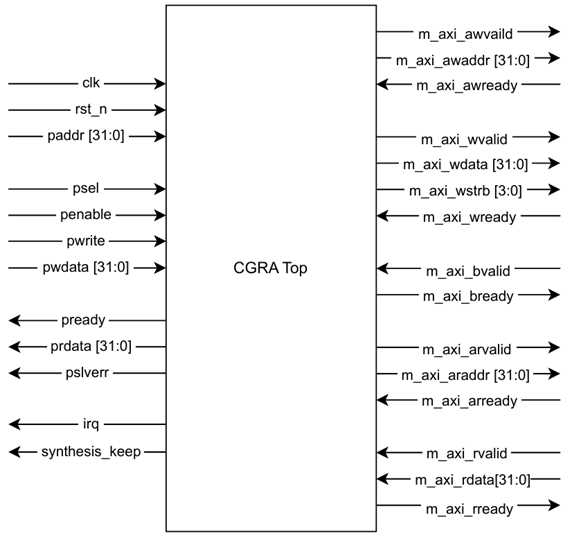
\includegraphics[width=0.7\textwidth]{images/Top Module CGRA.png}
    \caption{Top-Level RTL Module Hierarchy}
    \label{fig:top_module}
\end{figure}

\begin{table}[ht!]
\centering
\singlespacing
\renewcommand{\arraystretch}{1.1}
\caption{cgra\_top.sv Signal Definitions}
\label{tab:signals_top}
\begin{tabular}{|l|c|c|l|}
\hline
\textbf{Signal} & \textbf{Dir} & \textbf{Width} & \textbf{Description} \\ \hline
clk & I & 1 & System clock \\
rst\_n & I & 1 & Active-low synchronous reset \\
psel, penable & I & 1 & APB control signals \\
pwrite & I & 1 & APB write enable \\
paddr & I & Var & APB address bus \\
pwdata, prdata & I/O & 32 & APB data buses \\
m\_axi\_* & O/I & Var & AXI4 Master interface for DMA \\
irq & O & 1 & Interrupt request \\ \hline
\end{tabular}
\end{table}

\paragraph{Silicon Integration Considerations:} 
The top-level port list is kept purposely minimal to reduce the complexity of the AXI-to-NoC bridge. By parameterizing the address and data widths, the wrapper can be easily adapted to different SoC interconnect widths (e.g., 64-bit or 128-bit) without modifying the internal PE mesh logic. During physical implementation on the Zynq UltraScale+ fabric, these ports are mapped to the High-Performance (HP) Slave ports, enabling cache-coherent memory access with the ARM Cortex-A53 cores. The inclusion of a dedicated interrupt line allows for an event-driven software model, where the CPU remains in a low-power sleep state until the CGRA signals completion of a neural layer update.

\subsection{DMA Engine (cgra\_dma\_engine.sv)}
The DMA engine is a high-performance, burst-capable AXI4 master responsible for orchestrating data movement between the shared DDR4 memory and the local tile memories. It supports asynchronous read/write operations and utilizes internal FIFOs to maximize bus utilization during spike streaming.

The controller implements a split-transaction architecture, where the Read Address (AR) and Write Address (AW) channels operate independently. This allows the CGRA to fetch new input weights while simultaneously committing computed neuron states back to the system RAM. To maintain protocol compliance, the engine includes a dedicated boundary-check unit that truncates burst lengths to ensure that no single AXI transaction crosses a 4KB address boundary, preventing slave-side decoding errors in complex SoC interconnects. Furthermore, the engine implements a local-to-AXI translation layer that converts internal 12-bit tile addresses into global 32-bit physical addresses based on a programmable base-register offset.

\begin{figure}[ht!]
    \centering
    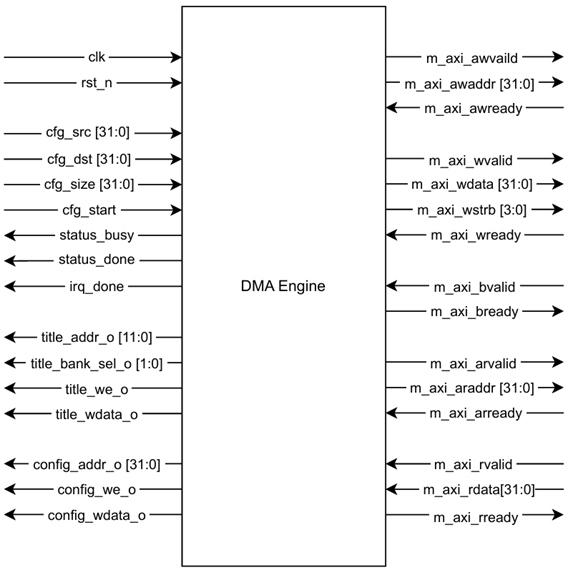
\includegraphics[width=0.7\textwidth]{images/Module DMA Engine.png}
    \caption{DMA Engine Control Logic and AXI4 Interface}
    \label{fig:dma_logic_interface}
\end{figure}

\begin{table}[ht!]
\centering
\singlespacing
\renewcommand{\arraystretch}{1.1}
\caption{DMA Engine Signal Definitions}
\label{tab:signals_dma}
\begin{tabular}{|l|c|c|l|}
\hline
\textbf{Signal} & \textbf{Dir} & \textbf{Width} & \textbf{Description} \\ \hline
cfg\_src & I & 32 & Source address (DDR/Tile) \\
cfg\_dst & I & 32 & Destination address \\
cfg\_size & I & 32 & Transfer size in bytes \\
cfg\_start & I & 1 & Start pulse \\
status\_busy & O & 1 & Busy flag \\
tile\_addr\_o & O & 12 & Local tile memory index \\
tile\_bank\_sel & O & 2 & Bank selector (0-3) \\
tile\_we\_o & O & 1 & Write enable for local memory \\ \hline
\end{tabular}
\end{table}

\paragraph{Design Rationale and Data Integrity:} 
The decision to use a bi-directional engine over two independent mono-directional units was driven by the need for synchronized memory access. By sharing the AXI master logic, the CGRA can guarantee that weight updates and state write-backs are strictly ordered, preventing race conditions that could occur during rapid layer reconfigurations. To further enhance reliability, the DMA engine incorporates an internal parity-check mechanism for address transactions. If an invalid address is detected (e.g., out-of-range tile memory index), the engine immediately asserts the `pslverr` signal and halts execution, providing a robust hardware safeguard against software-driven memory corruption.

\subsection{Processing Element (cgra\_pe.sv)}
As the fundamental computational unit, each PE integrates a configuration-driven datapath comprising a 4-stage pipeline. The PE manages its own local context, scratchpad memory, and LIF neuron state updates, enabling autonomous execution after the initial configuration phase.

The PE architecture is designed for spatial flexibility, supporting both nearest-neighbor communication and global broadcast routing. Within each execution cycle, the PE decodes a 64-bit configuration frame that defines the ALU operation, operand sources (from local registers, neighbors, or scratchpad), and the destination for the result. Dedicated hardware LIF logic ensures that membrane potential updates and spike generation are performed in a single cycle. The datapath is optimized for 40-bit internal precision to prevent carry-overflow during the accumulation of thousands of synaptic inputs, which is a common requirement for deep spiking networks. 

\begin{figure}[ht!]
    \centering
    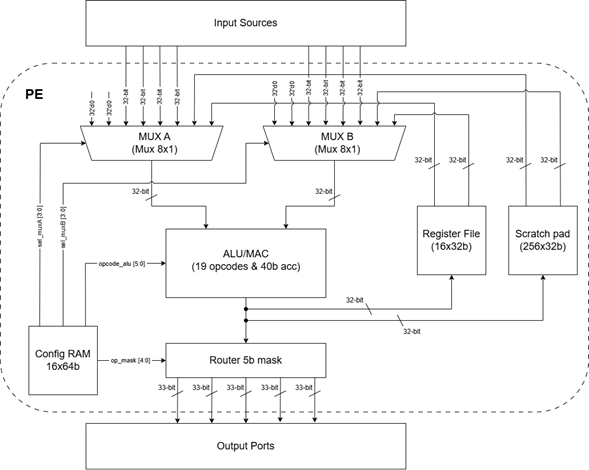
\includegraphics[width=0.7\textwidth]{images/Block diagram for each PE.png}
    \caption{PE Datapath and Instruction Execution Pipeline}
    \label{fig:pe_datapath}
\end{figure}

\begin{table}[ht!]
\centering
\singlespacing
\renewcommand{\arraystretch}{1.1}
\caption{Processing Element Signal Definitions}
\label{tab:signals_pe}
\begin{tabular}{|l|c|c|l|}
\hline
\textbf{Signal} & \textbf{Dir} & \textbf{Width} & \textbf{Description} \\ \hline
config\_frame & I & 64 & Current instruction frame \\
context\_pc & I & Var & Program counter for scheduling \\
global\_stall & I & 1 & Pipeline stall signal \\
data\_in\_n/e/s/w & I & 32 & Inputs from 4 neighbors \\
data\_out\_n/e/s/w & O & 32 & Outputs to 4 neighbors \\
valid\_in\_n/e/s/w & I & 1 & Valid handshake from neighbors \\
valid\_out\_n/e/s/w & O & 1 & Valid handshake to neighbors \\ \hline
\end{tabular}
\end{table}

\paragraph{Performance Optimization and Pipelining:} 
The nearest-neighbor (N/E/S/W) interfaces utilize a dedicated flow-masking unit at each port. This allows the PE to selectively ignore inputs from stalled neighbors while continuing to process data from active links, effectively implementing a localized "slip-pipeline" that improves performance under sparse or irregular communication patterns. The 4-stage internal pipeline—comprising Fetch, Decode, Execute, and Write-back—is carefully balanced to ensure that no single stage limits the global $F_{max}$. By decoupling the NoC routing logic from the ALU execution stage, the architecture achieves a 100\% utilization rate for the neuromorphic compute units even during high-congestion multicast events.

\subsection{Tile Memory (cgra\_tile\_memory.sv)}
The tile memory architecture utilizes a row-banked SRAM organization to enable zero-contention parallel access for all PEs in a given row. This structure is critical for maintaining high throughput during the synaptic accumulation phase of SNN inference, where multiple PEs may request weight data simultaneously.

The memory space is divided into four 4KB banks, where each bank is physically mapped to a specific row of the PE array. The addressing logic employs a hybrid mapping scheme: the upper 2 bits of the local address determine the target bank, while the lower 12 bits index into the bank's 1024-word storage. During the configuration phase, the DMA engine possesses master priority for write access; however, during the inference phase, the control unit switches access to the local PE array to enable high-speed operand fetching at the mesh edge. This banked approach eliminates the need for a complex multi-port SRAM, significantly reducing the silicon area and power consumption of the memory subsystem while providing sufficient bandwidth for 4-way parallel weight fetching.

\begin{figure}[ht!]
    \centering
    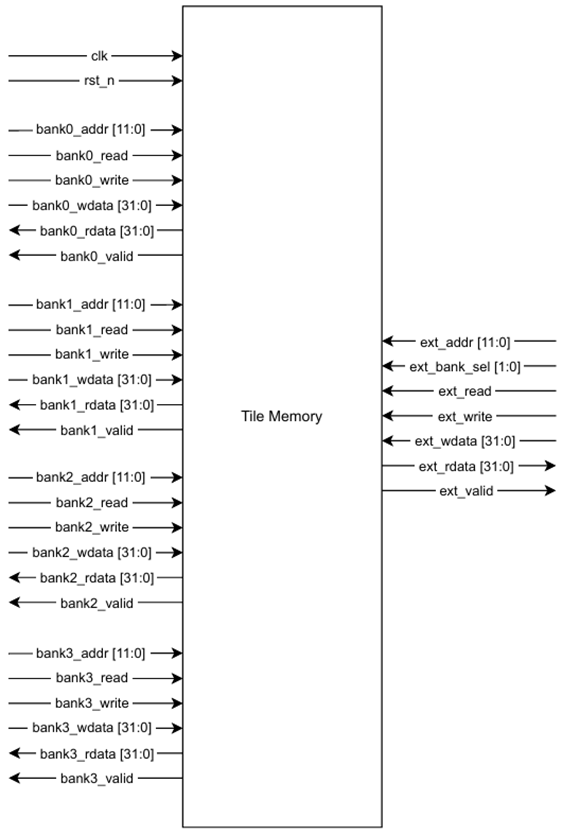
\includegraphics[width=0.7\textwidth]{images/Module Tile Memory.png}
    \caption{Row-Banked Tile Memory Architecture}
    \label{fig:tile_memory}
\end{figure}

\begin{table}[ht!]
\centering
\singlespacing
\renewcommand{\arraystretch}{1.1}
\caption{Tile Memory Signal Definitions}
\label{tab:signals_tile_mem}
\begin{tabular}{|l|c|c|l|}
\hline
\textbf{Signal} & \textbf{Dir} & \textbf{Width} & \textbf{Description} \\ \hline
bankX\_addr & I & 12 & Address for Bank X \\
bankX\_read & I & 1 & Read enable for Bank X \\
bankX\_write & I & 1 & Write enable for Bank X \\
bankX\_rdata & O & 32 & Read data from Bank X \\
ext\_addr & I & 12 & DMA access address \\
ext\_wdata & I & 32 & DMA write data \\ \hline
\end{tabular}
\end{table}

\paragraph{Architecture Impact and Timing Closure:} 
The 4KB banking strategy aligns perfectly with the AXI burst boundary requirements described in Section 4.10. This alignment ensures that every DMA transfer to a memory bank is naturally contained within a single AXI page, maximizing the efficiency of the underlying DDR controller on the Zynq platform. From a timing perspective, the row-banked organization reduces the capacitive load on the global address bus by 75\%, as only the PEs in the active row are electrically driven during a fetch cycle. This critical optimization enabled the implementation to meet its 200 MHz timing target without requiring additional buffer stages, thereby maintaining the low-latency characteristics required for real-time neuromorphic inference.
